\documentclass[fr]{../../../../../../eplexam}
\usepackage[utf8]{inputenc}
\usepackage{tikz}
\usepackage{float}
\usepackage{enumitem}
\usepackage{circuitikz}
\usepackage{subcaption}
\usepackage{multicol}
\usepackage{../../../../../../eplunits} 


\hypertitle{Projet Elec}{4}{ELEC}{1101}{2018}{Juin}{Majeure}
{Quentin Dessain}
{Christophe Craeye, Bruno Dehez et Claude Oestges}


\makeatletter
\@addtoreset{section}{part}
\makeatother

\begin{center}
Les questions et réponses de ce document ne sont nullement officielles. Des différences peuvent exister entre l'examen réel et ce correctif. Les réponses présentes ci-dessous sont uniquement basées sur les réponses de l'auteur durant l'examen et ne sont donc pas nécessairement valides.
\end{center}

\part{QCM}

\section{Lors du projet, le signal reçu après la réception était souvent de l'ordre de quelques milli-volts. On veut amplifier avec un gain de 10 000 un signal reçu comportant des paquets d'onde à une fréquence de 40KHz à l'aide de TL084/TL082. Quelle est la proposition correcte :}

\begin{enumerate}[label=(\alph*)]
    \item Il faut utiliser un amplificateur inverseur
    \item Il faut utiliser un amplificateur non-inverseur
    \item Tout les montages d'amplification fonctionnent
    \item C'est impossible de réaliser cela à l'aide d'amplificateur
    \item Il faut utiliser deux amplificateurs opérationnels
    \item Aucune des propositions ci-dessus ne sont correctes
\end{enumerate}
\vspace{-0.5cm}
\begin{solution}
Le produit GBP dans un TL084 et TL082 est typiquement de $4MHz$ (cf. datasheet). Vu que le signal est à une fréquence de 40kHz, le gain maximum par amplificateur est d'environ $\frac{4 000 000}{40 000}=100$. Un seul amplificateur ne convient donc pas. Deux amplificateurs en série conviennent, car le produit de leur gain est égale à 10 000 ($100*100=10 000$). Idéalement en pratique, il faut trois amplificateurs en série pour pouvoir amplifier sans dépasser le produit GBP et avoir un minimum de marge. La réponse est donc la E.
\end{solution}

\section{Un amplificateur inverseur idéal a:}

\begin{figure}[H]
    \centering
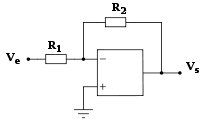
\includegraphics[scale=1]{inverseur.png}
    \caption{Amplificateur Inverseur}
    \label{fig:my_label}
\end{figure}

\begin{multicols}{2}
Une impédance de sortie égale à:
\begin{enumerate}[label=(\Alph*)]
    \item Infinie
    \item Nulle
    \item R1
    \item R2
    \item R1+R2
    \item R1\textbackslash\textbackslash R2
\end{enumerate}
\columnbreak
Une impédance d'entrée égale à:
\begin{enumerate}[label=(\alph*)]
    \item Infinie
    \item Nulle
    \item R1
    \item R2
    \item R1+R2
    \item Dépendante de la charge $Z_L$ situé en sortie de l'inverseur.
\end{enumerate}
\end{multicols}
\vspace{-0.5cm}
\begin{solution}
Impédance d'entrée: R1 Impédance de sortie: Nulle (pas R2 car aop idéal)
\end{solution}


\section{Ci-dessous sont représentés un signal d'entrée et une série de signaux de sortie. Choisissez pour chacun des monostables le bon signal de sortie en fct du signal d’entrée.}

\begin{figure}[H]
    \centering
\begin{subfigure}[b]{0.49\textwidth}
\centering
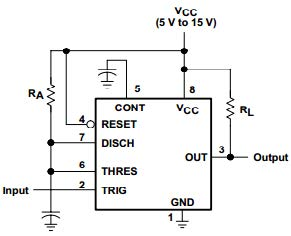
\includegraphics[width=\linewidth]{Monostable_NE555.jpg}
\caption{Monostable avec NE555}
\end{subfigure}
\begin{subfigure}[b]{0.50\textwidth}
\centering
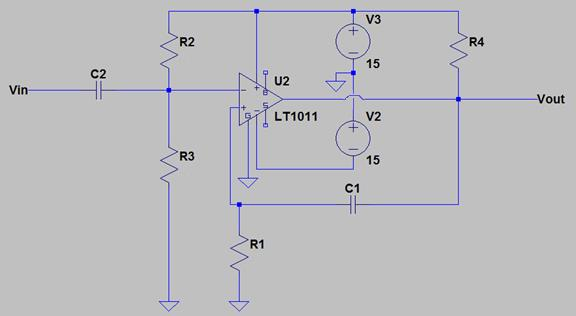
\includegraphics[width=\linewidth]{Monostable_LM319.jpg}
\caption{Monostable avec LM319}
\end{subfigure}
\end{figure}

Indiquez dans la grille de réponse la lettre correspondant au signal de sortie du montage avec NE555 suivi de la lettre correspondant au signal de sortie du montage avec LM319. Exemple: AA, BC, DA 

\begin{figure}[H]
    \centering
\centerline{
\begin{subfigure}[b]{0.6\linewidth}
\centering
\centerline{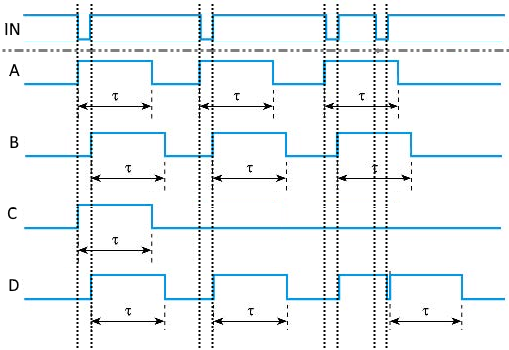
\includegraphics[width=\linewidth]{Monostable_g2.png}}
\end{subfigure}
\begin{subfigure}[b]{0.6\linewidth}
\centering
\centerline{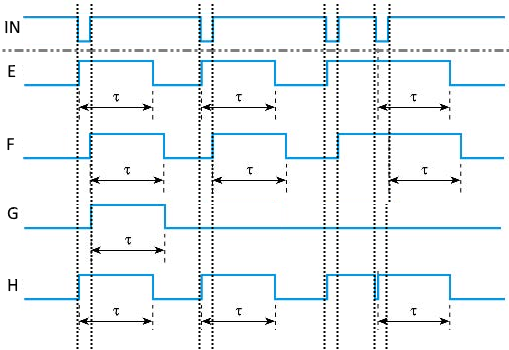
\includegraphics[width=\linewidth]{Monostable_g1.png}}
\end{subfigure}
}
\end{figure}

\begin{solution}
Le LM319 va trigger sur le flanc descendant du signal d'entrée. Il n'est pas retriggerable.
Le NE555 n'est pas non plus retriggerable et se déclenche également sur le flanc descendant. 
La seule différence entre les deux montages est que le montage avec NE555 va pouvoir prendre plus régulièrement des impulsions en entrée.
Le signal A correspond au NE555 et le signal C correspond au LM319.
\end{solution}

\section{Voici une représentation d'un montage typique situé en sortie d'un télémètre à ultrason. Sachant que l'impédance interne du switch est de $50m\si{\ohm}$. Quelle modification doit être apportée au montage pour qu'il fonctionne de façon appropriée.}

\begin{figure}[H]
    \centering
\begin{circuitikz}
\draw (2,2.5) -- (4,2.5) node[anchor=west] {In};
\draw (2,0) -- (4,0) node[anchor=west] {Ctrl};
\draw (9,2.5) -- (6,2.5) node[anchor=east] {Out};
\draw (7,2.5) to[capacitor] (7,1) node[cground]{};
\draw (4,-0.5) rectangle (6,3);
\end{circuitikz}
    \caption{Montage erroné}
    \label{fig:my_label}
\end{figure}
Quel montage ci-dessous est approprié ?
\begin{figure}[H]
\captionsetup[subfigure]{justification=centering}

\begin{subfigure}[b]{0.50\textwidth}
\resizebox{\linewidth}{!}{
\centering
\begin{circuitikz}
\draw (2,2.5) -- (4,2.5) node[anchor=west] {In};
\draw (2,0) -- (4,0) node[anchor=west] {Ctrl};
\draw (9,2.5) -- (6,2.5) node[anchor=east] {Out};
\draw (7,2.5) to[capacitor] (7,1) node[cground]{};
\draw (8,2.5) to[R] (8,1) node[cground]{};
\draw (4,-0.5) rectangle (6,3);
\end{circuitikz}
}
\caption{}
\end{subfigure}
\begin{subfigure}[b]{0.50\textwidth}
\centering
\resizebox{\linewidth}{!}{
\begin{circuitikz}
\draw (2,2.5) -- (4,2.5) node[anchor=west] {In};
\draw (2,0) -- (4,0) node[anchor=west] {Ctrl};
\draw (9,2.5) -- (6,2.5) node[anchor=east] {Out};
\draw (7,2.5) to[capacitor] (7,1) node[cground]{};
\draw (3,2.5) to[R] (3,1) node[cground]{};
\draw (4,-0.5) rectangle (6,3);
\end{circuitikz}
}
\caption{}
\end{subfigure}
%
\begin{subfigure}[b]{0.50\textwidth}
\centering
\resizebox{\linewidth}{!}{
\begin{circuitikz}
\draw (2,2.5) -- (4,2.5) node[anchor=west] {In};
\draw (3,0) to[R] (3,1.5) node[rotate=180,cground]{};
\draw (2,0) -- (4,0) node[anchor=west] {Ctrl};
\draw (9,2.5) -- (6,2.5) node[anchor=east] {Out};
\draw (7,2.5) to[capacitor] (7,1.5) node[cground]{};
\draw (4,-0.5) rectangle (6,3);
\end{circuitikz}
}
\caption{}
\end{subfigure}
\begin{subfigure}[b]{0.50\textwidth}
\centering
\resizebox{\linewidth}{!}{
\begin{circuitikz}
\draw (2,2.5) -- (4,2.5) node[anchor=west] {In};
\draw (2,0) to[R] (4,0) node[anchor=west] {Ctrl};
\draw (9,2.5) -- (6,2.5) node[anchor=east] {Out};
\draw (7,2.5) to[capacitor] (7,1.5) node[cground]{};
\draw (4,-0.5) rectangle (6,3);
\end{circuitikz}
}
\caption{}
\end{subfigure}
%
\begin{subfigure}[b]{0.50\textwidth}
\centering
\resizebox{\linewidth}{!}{
\begin{circuitikz}
\draw (2,2.5) to[R] (4,2.5) node[anchor=west] {In};
\draw (2,0) -- (4,0) node[anchor=west] {Ctrl};
\draw (9,2.5) -- (6,2.5) node[anchor=east] {Out};
\draw (7,2.5) to[capacitor] (7,1.5) node[cground]{};
\draw (4,-0.5) rectangle (6,3);
\end{circuitikz}
}
\caption{}
\end{subfigure}
\begin{subfigure}[b]{0.50\textwidth}
\centering
\resizebox{\linewidth}{!}{
\begin{circuitikz}
\draw (3,2.5) -- (3,3.5) to[R] (6.5,3.5) -- (6.5,2.5);
\draw (2,2.5) -- (4,2.5) node[anchor=west] {In};
\draw (2,0) -- (4,0) node[anchor=west] {Ctrl};
\draw (9,2.5) -- (6,2.5) node[anchor=east] {Out};
\draw (7,2.5) to[capacitor] (7,1.5) node[cground]{};
\draw (4,-0.5) rectangle (6,3);
\end{circuitikz}
}
\caption{}
\end{subfigure}

\end{figure}

\begin{solution}
La solution est la e. C'est la seul qui permet de limiter le courant entrant dans le switch sans changer le comportement du montage.
\end{solution}


\section{Dans le cadre du projet, un montage basé sur un amplificateur opérationnel est utilisé pour générer un signal carré. La sortie du montage est reliée à une résistance de charge de $1\si{\ohm}$. Malheureusement le montage ne fonctionne pas. Quelle est la caractéristique non idéale de l'amplificateur opérationnel \textbf{la plus critique} qui empêche le bon fonctionnement du montage?}

\begin{enumerate}[label=(\alph*)]
    \item Les courants de polarisation
    \item Le taux de rampe limité
    \item La tension de saturation
    \item La tension d'offset
    \item La limitation du courant de sortie
    \item Aucune des réponses précédentes
\end{enumerate}

\begin{solution}
Vu que la résistance de charge est très faible, l'aop va devoir délivrer beaucoup (trop) de courant. C'est donc principalement la limitation du courant de sortie qui va empêcher le bon fonctionnement du montage.
\end{solution}


\section{On souhaite augmenter la longueur maximale de mesure d'un télémètre à ultrason standard. Quelle modification a du sens?}

\begin{enumerate}[label=(\alph*)]
    \item Augmenter le nombre de périodes du signal à $40kHz$ envoyé
    \item Diminuer le nombre de périodes du signal à $40kHz$ envoyé
    \item Augmenter la fréquence des mesures
    \item Diminuer la fréquence des mesures
    \item Diminuer le temps durant lequel la réception directe est bloquée
    \item Diminuer la tension d'alimentation
    \item Aucune des propositions ci-dessus
\end{enumerate}

\begin{solution}
L'unique solution allant dans le bon sens est de diminuer la fréquence de mesures. Pour information, diminuer le temps durant lequel la réception directe est bloquée ne permet pas de mesurer plus loin mais plus proche.
\end{solution}

\section{On souhaite afficher à l'oscilloscope la prise de mesure d'un signal à une fréquence de $40kHz$, d'une amplitude de $1V$ et d'un offset de $500mV$. Voici une photo du résultat affiché à  l'oscilloscope. Sur quel bouton devra-t-on appuyer au minimum pour pouvoir correctement afficher le signal?}

\begin{figure}[H]
    \centering
    \centerline{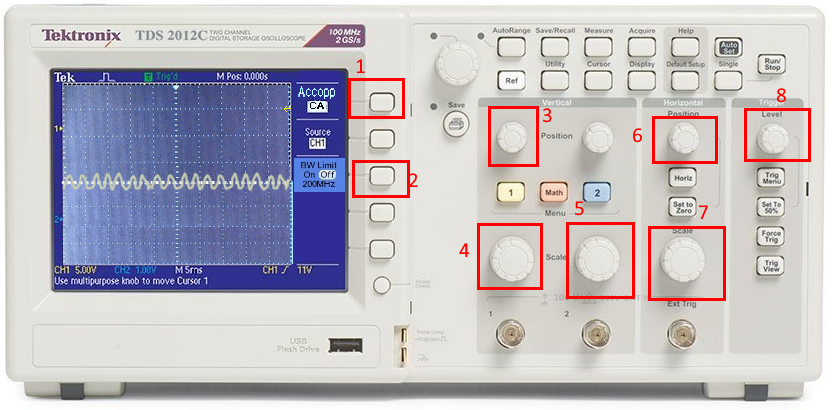
\includegraphics[width=1.2\linewidth]{scope.png}}
    \caption{Oscillioscope}
    \label{fig:my_label}
\end{figure}

\begin{multicols}{3}
\begin{enumerate}[label=(\alph*)]
    \item 1,2,3,4,8
    \item 3,4
    \item 3,4,7
    \item 4,7
\columnbreak
    \item 1,4,7,8
    \item 4,7,8
    \item 3,4,7
    \item 1,2,3,4,5,6,7,8
\columnbreak
    \item 1,2,4,7
    \item 2,4,7
    \item 2,3,5
    \item 2,3,4
\end{enumerate}
\end{multicols}

\begin{solution}
La séquence 1,4,7,8 permet d'afficher le signal de façon optimale. Le bouton 1 fait passer l'oscilloscope en mode DC afin de pouvoir visualiser l'offset, le bouton 4 permet d'ajuster l'échelle verticale (qui est initialement à $5 V/div$), le bouton 7 permet d'ajuster l'échelle horizontale et le bouton 8 sert à diminuer la tension de trigger.  
\end{solution}

\section{Afin de faciliter l'ajustement de son montage. Un étudiant a décidé de placer un potentiomètre sur le montage générateur ci-dessous, quel est le rôle de ce dernier? Le potentiomètre est situé dans le carré sur le schéma ci-dessous.}
%https://perso.esiee.fr/~poulichp/PR201/OSC_carre/OSC_Carre.html

\begin{figure}[H]
\centering
\begin{circuitikz}
\draw (0,0) node[op amp]{};
\draw (-1,-0.5) -- (-1.5,-0.5) -- (-1.5,-1.5) to[R] (-1.5,-3) node[cground]{};
\draw (-1.5,-1.5) to[R] (1.5,-1.5) -- (1.5,2.2);
\draw (1,0) -- (2,0) node[anchor=west]{$V_{out}$};
\draw (-1,0.5) -- (-2.5,0.5) -- (-2.5,-1.5) to[capacitor] (-2.5,-3) node[cground]{};
\draw (-2.5,1.5)-- (-2.5,2.9) to[R] (-0.5,2.9) to[Do] (1,2.9) to[american potentiometer] (1,1.5) to[Do] (-0.5,1.5) to[R] (-2.5,1.5) -- (-2.5,-1.5);
\draw (-0.5,1) rectangle (1.8,3.4);
\end{circuitikz}
\caption{Générateur Signal Carré}
\end{figure}


Rôle du potentiomètre:
\begin{enumerate}[label=(\alph*)]
    \item Changer la tension de basculement
    \item Changer l'amplitude du signal
    \item Changer le rapport cyclique du signal
    \item Changer la fréquence du signal
    \item Aucune des propositions précédentes
\end{enumerate}

\begin{solution}
Modifier le potentiomètre change le temps de chargement et déchargement de la capacité tout en gardant le temps totale constant. Cela modifie donc le rapport cyclique. 
\end{solution}



\pagebreak






\part{Question ouverte}


\begin{figure}[H]
    \centering
   \centerline{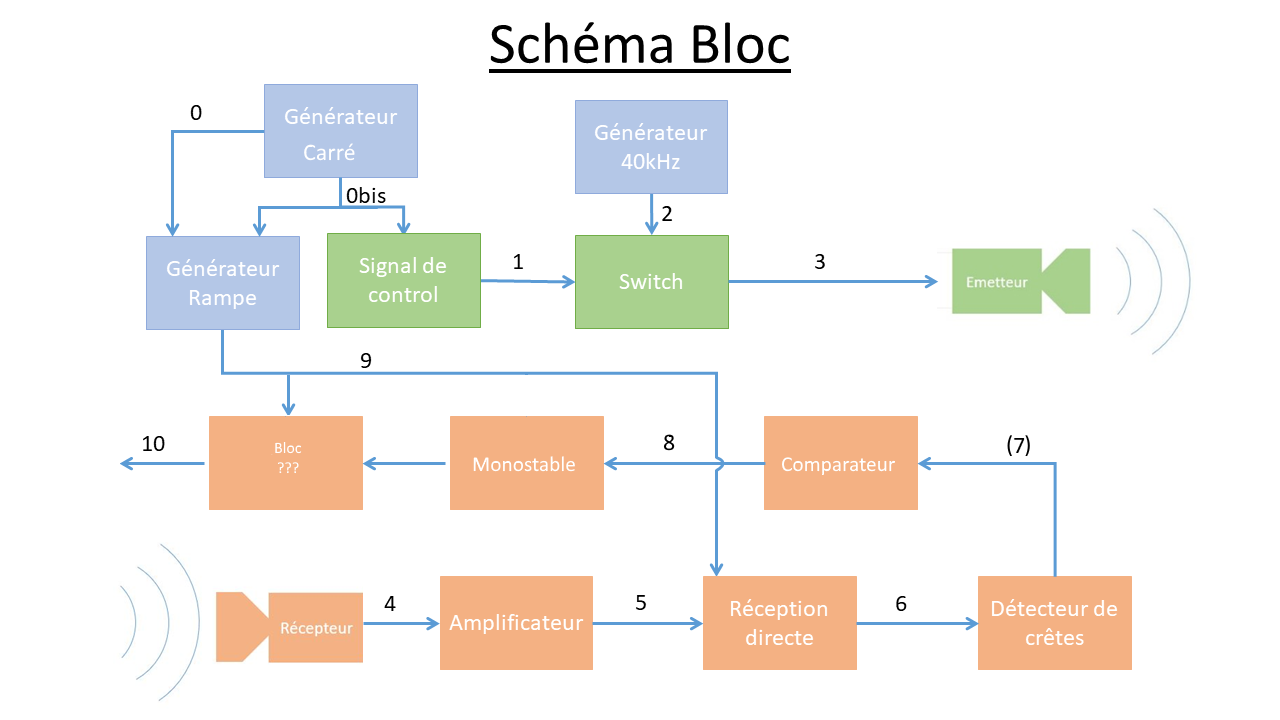
\includegraphics[width=1.2\linewidth]{Schema_bloc.png}}
    \caption{Schéma Bloc}
    \label{fig:sch_bloc}
\end{figure}

\begin{figure}[H]
    \centering
		\vspace{-1cm}
    \centerline{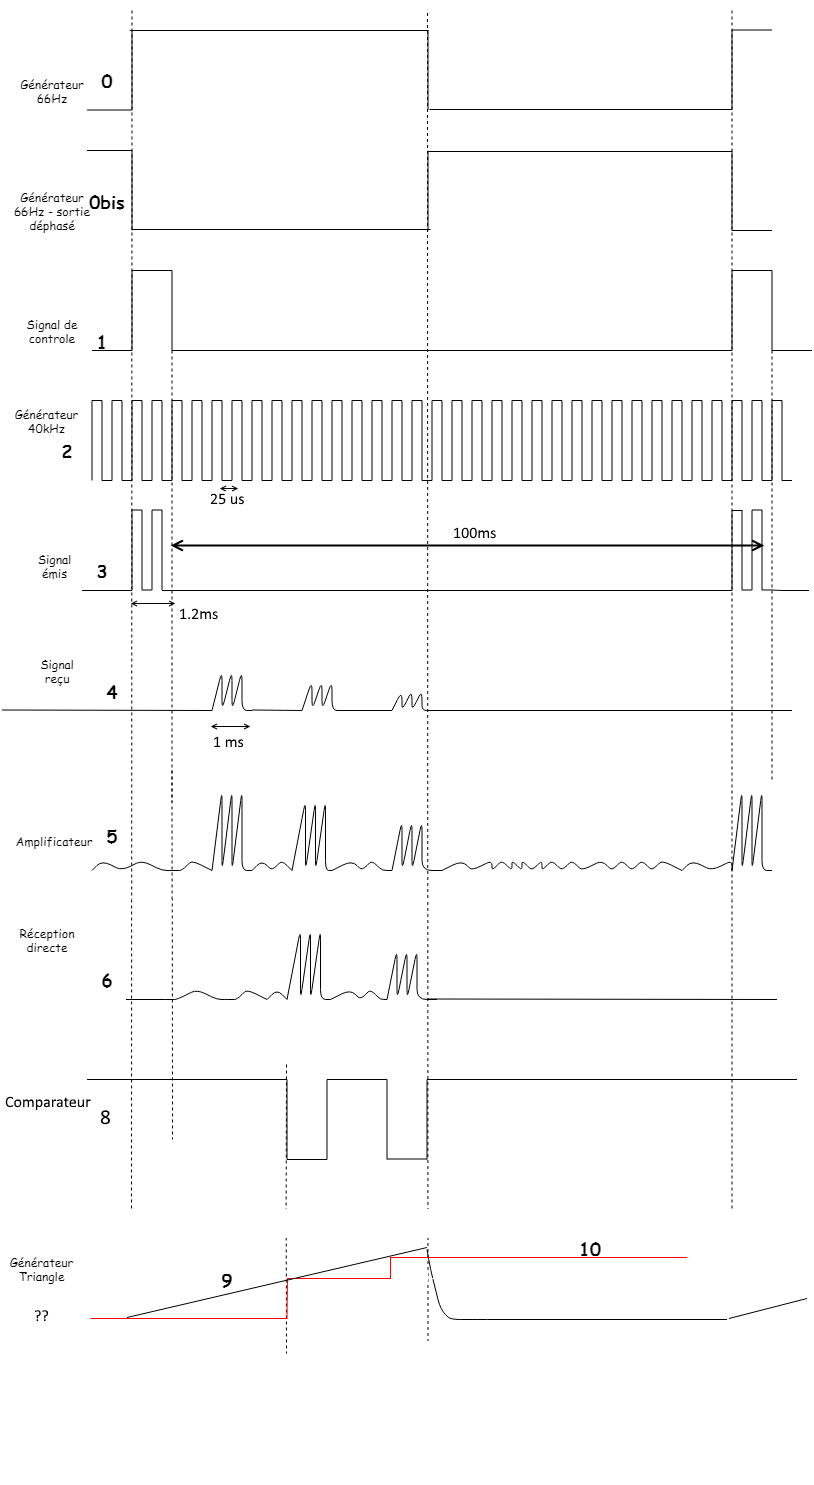
\includegraphics[width=1\linewidth,height=1.1\textheight]{tableau_signaux.png}}
    \caption{Tableau des signaux}
    \label{fig:tab}
\end{figure}

\section{Quel est le nom typique du bloc "???" sur la figure \ref{fig:sch_bloc}? Donner son implémentation circuit.}

\begin{solution}
Le bloc est un "sample and hold".
Son implémentation circuit est la suivante:
\begin{figure}[H]
    \centering
    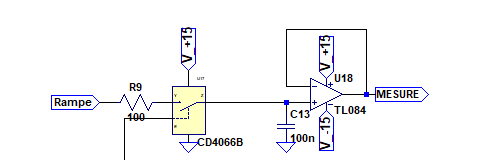
\includegraphics[width=\textwidth]{sampleandhold.png}
\end{figure}
\end{solution}

\section{Donner l'implémentation circuit du détecteur de crête (passif) et expliquer son fonctionnement}

\begin{solution}
Son implémentation circuit est la suivante:
\begin{figure}[H]
    \centering
    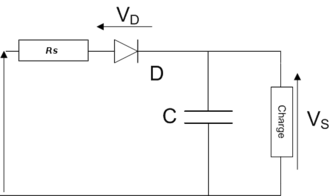
\includegraphics{detecteur_passif.png}
\end{figure}
Lorsqu'un signal va arriver en entrée, la capaciter va se charger. Par contre lorsque le signal va osciller rapidement, la capacité va seulement se décharger très faiblement à cause de sa cst de temps bien supérieur à la fréquence d'oscillation. Lorsqu'il n'y a plus de signal en entrée, la capacité va pouvoir se décharger. Cela a pour effet d'envelopper le signal.
\end{solution}

\section{Dessiner sur le signal en sortie de la réception directe sur la fig \ref{fig:tab} l'allure de la sortie du détecteur de crête}

\begin{solution}
\begin{figure}[H]
    \centering
    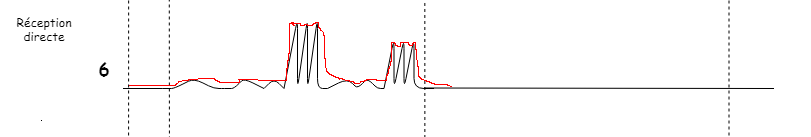
\includegraphics{crete.png}
\end{figure}
\end{solution}

\section{Quelle non-idéalité/désavantage comporte ce détecteur de crête ? Proposer une solution (peu utiliser des éléments actifs).}

\begin{solution}

\begin{figure}[H]
    \centering
    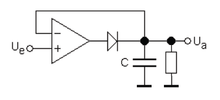
\includegraphics{detecteur_actif.png}
		\caption{Detecteur avec super diode}
\end{figure}

Le seuil de basculement de la diode est de $\approx 0.7$Volt, ce qui empêche la détection de signaux de faible amplitude. De plus, la crête sera systématiquement $\approx0.7$ volt moins élevé que $Vmax$. Utiliser une super diode (qui a un seuil de basculement valant $\frac{\approx 0.7}{gain de l'oaop}$) résous ce problème.

\begin{figure}[H]
    \centering
    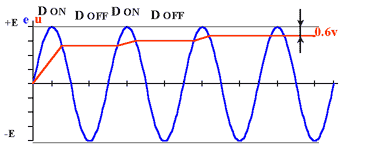
\includegraphics{crete_graph.png}
    \caption{Illustration}
\end{figure}
\end{solution}

\section{Dimensionner le détecteur de crête dans un cas générale en fct d’un signal d’entrée générale}

\begin{solution}
De façon qualitative, la cst de temps de la capacité doit être plus grande que la fréquence d'oscillation du signal d'entrée. La résistance doit quant à elle ne pas être trop faible pour éviter que trop de courant "ne parte" au travers de la résistance. Par contre la cst de temps doit être bcp plus faible que la fréquence porteuse du signal.
\end{solution}


\vspace{1cm}

Le schéma bloc de la figure \ref{fig:sch_bloc} ne traite pas le cas ou des réflexions multiples sont captés.

\section{Vous disposer d’un signal de reset, améliorer le détecteur de crête à l’aide de composants utilisés en laboratoire pour que la sortie du détecteur de crête soit nulle lorsque le signal de reset est non nul.}

\begin{solution}
Une solution est de placer un switch commandé par le signal de reset à la sortie du détecteur de crête. 
\end{solution}

\section{Comment pourriez-vous utiliser cette implémentation pour supprimer la réflexion multiple ? Expliquer son fonctionnement et dessiner l’allure des signaux.}

\begin{solution}
Après la première impulsion dépassant le seuil de mesure du comparateur, le signal de reset passerait à 1 et bloquerait les impulsions suivantes. Ce signal de reset peut par exemple être généré à l'aide d'un monostable rettrigerable qui se réinitialiserait à la fin d'une période de mesure juste avant l'émission suivante.
\begin{figure}[H]
    \centering
    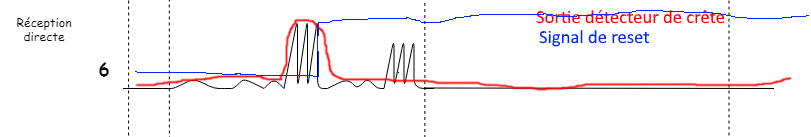
\includegraphics[width=\textwidth]{refl_mult.png}
\end{figure}
\end{solution}

\section{À l’aide des graphes de la figure \ref{fig:tab}, dimensionner le détecteur de crête.}
\begin{solution}
On peut par exemple prendre une capacité de 20nF et une résistance de 10k.
\end{solution}

\end{document}
